%TODO in generale mettere la citazione quando si parla di qualcosa in tutta la sezione

As introduced before, the simple strategy of classifying views independently works remarkably well, but the focus of this section is to explain new ideas for how to “compile” the information in multiple 2D views of an object into a compact object descriptor using a new architecture called multi-view CNN. The multi-view CNN learns to combine the views instead of averaging, and thus can use the more informative views of the object for prediction while ignoring others. The multi-view approach, in the image classification context, is related to “jittering” (or data augmentation) as the different views can be seen as jittered copies. The method that will be described in fact can be also applied to jittered copies and can outperforms standard CNNs trained with the same jittered copies (for example on the sketch recognition benchmark~\cite{eitz2012hdhso}).

Let's start from the data: the view-based representations start from multiple views of a 3D shape, generated by a rendering engine. As said before, we could simply average the descriptors obtained from these views (that are all considered equally important) and obtain good results. Another approach is to concatenate all the different views and obtain a single big compact descriptor, but in this case we need to always respect the same point of views order and applying this order is not always possible, because the pose of the objects must be the expected one or correctly deduced.
The approach we'll describe, instead, learns to combine information from multiple views using a unified CNN architecture that includes a view-pooling layer.

\paragraph{Input}
In order to generate the different views of a 3D object, given its point cloud representation, we essentially need to preprocess the data with two steps: 
we connect the points and obtain edges forming faces (not necessary if the 3D models in the database is stored as polygon meshes) and in order to generate rendered views of
polygon meshes we need to use a reflection model (in the described approach is used the the Phong reflection model). Next we can apply the perspective projection and uniformly scale shapes to fit into the viewing volume. 
Two different cameras setup were experimented:\begin{itemize}
\item {\textbf{Camera setup 1: } is assumed that the input shapes are upright oriented, as the most online database are. 12 cameras, each every 30 degrees, elevated 30 degrees from the ground plane point toward the centroid of the mesh. See the left side of figure \ref{fig:multiview}.}
\item {\textbf{Camera setup 2: } the previous assumption about the upright orientation is eliminated so we need more views to ensure a good representation. 20 cameras pointing toward the centroid of the mesh are placed at the 20 vertices of an icosahedron enclosing the shape. Then, for each camera is taken a view using 0, 90, 180, 270 degrees rotation along the axis passing through the camera and the object centroid. This camera setup therefore has a total of 80 views.}
\end{itemize}

\begin{figure}[ht]
    \centering
    \captionsetup{width=.8\linewidth}
    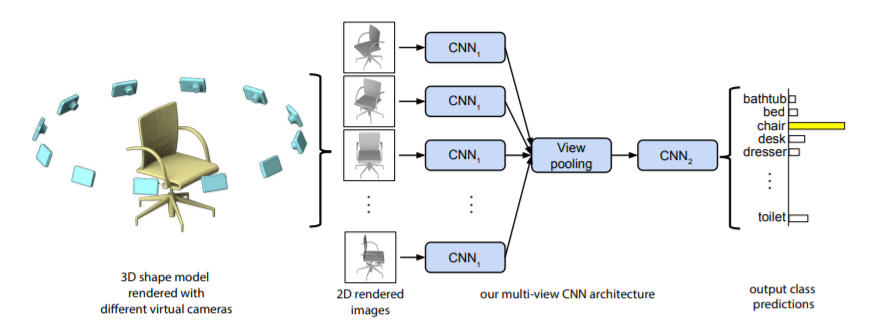
\includegraphics[width=0.8\textwidth]{images/multiview.png}
    \caption{ Multi-view CNN for 3D shape recognition (illustrated using the 1st camera setup). At test time a 3D shape is rendered from 12
different views and are passed thorough CNN1 to extract view based features. These are then pooled across views and passed through
CNN2 to obtain a compact shape descriptor.}
    \label{fig:multiview}
\end{figure}

\paragraph{Architecture}
\textbf A simple approach is to fine-tune a pre-trained CNN using the different views, obtaining a descriptor for each view. Then we train one-vs-rest linear SVMs (each view is treated as a separate training sample) to classify shapes using their image features. At test time, we simply sum up the SVM decision values over all 12 views and return the class with the highest sum. Alternative approaches like averaging image descriptors, lead to worse accuracy.

Let's describe now an approach that  \textbf{learns to aggregate views: MVCNN}. The input of the network are the different views of the 3D object. Each of these views is passed through the the first part of the network (CNN1) that is formed by 5 convolutional layers. Consequently the quantity of branches is equal to the quantity of views. The feature maps in output from this part are then aggregated at a viewpooling layer into a single feature map. At the end of the architecture (CNN2) we have 3 fully connected layers. See figure \ref{fig:mvcnn} to visualize the structure and table \ref{fig:MVCNN_TABLE} for layers details.

\begin{figure}[ht]
    \centering
    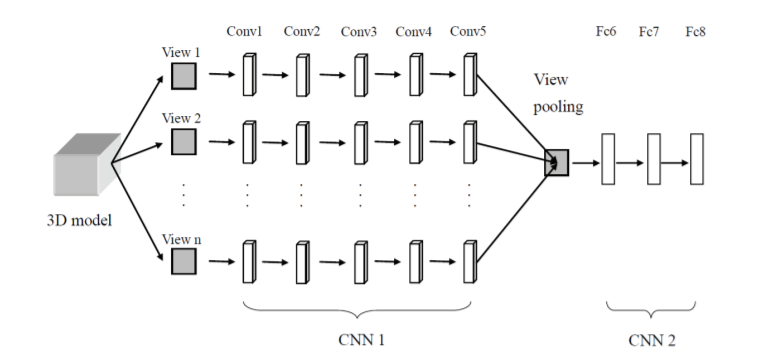
\includegraphics[width=0.8\textwidth]{images/mvcnn.png}
    \caption{Architecture of MVCNN model.}
    \label{fig:mvcnn}
\end{figure}

\begin{figure}[ht]
    \centering
    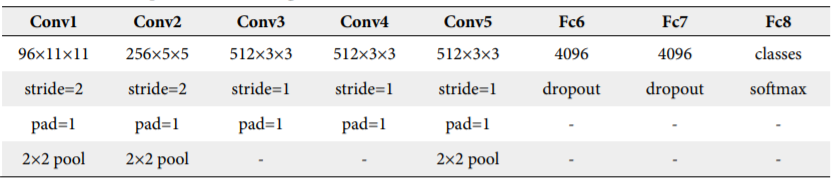
\includegraphics[width=0.8\textwidth]{images/MVCNN_TABLE.png}
    \caption{ Details on parameters of the MVCNN.}
    \label{fig:MVCNN_TABLE}
\end{figure}
\newpage

All branches in the first part of the network share the same parameters in CNN1. The view-pooling layer uses element-wise max pooling strategy to combine the discriminative information of multiple views and increase the computational efficiency. The viewpooling method is similar to traditional max-pooling operation. An alternative is element-wise mean
operation, but it is not as effective. The view-pooling layer can be placed anywhere in the network but experiments show that setting it after the 5th convolutional layer is the best choice. The MVCCN is fine-tuned for classification, but using a Mahalanobis metric W that directly projects the output descriptor $\phi \in \mathbb{R}^d$ to $W(\phi) \in \mathbb{R}^p$ and calculating the $l_2$ distance in the projected space we obtain a significant boost to retrieval performance.

An MVCNN can also be used as a simple 2D image classifier instead of CNN. If we use data augmentation and feed the MVCNN with all the different jittered copies and the original image we can obtain better results than using a CNN (experiments are reported in ~\cite{multi_view} on the sketch recognition benchmark~\cite{eitz2012hdhso}).

\paragraph{Results}
The dataset used is ModelNet40, described in section \ref{ModNet40}. The table in figure \ref{fig:MVCNN_results_table} compares different settings of MVCNNs to other approaches like SPH(Spherical Harmonics descriptor), LFD (LightField descriptor) and 3D ShapeNets on the ModelNet40 dataset. See also the retrieval precision-recall curves in figure \ref{fig:MVCNN_prec_rec_curve}.

\begin{figure}[ht]
    \centering
    \captionsetup{width=.8\linewidth}
    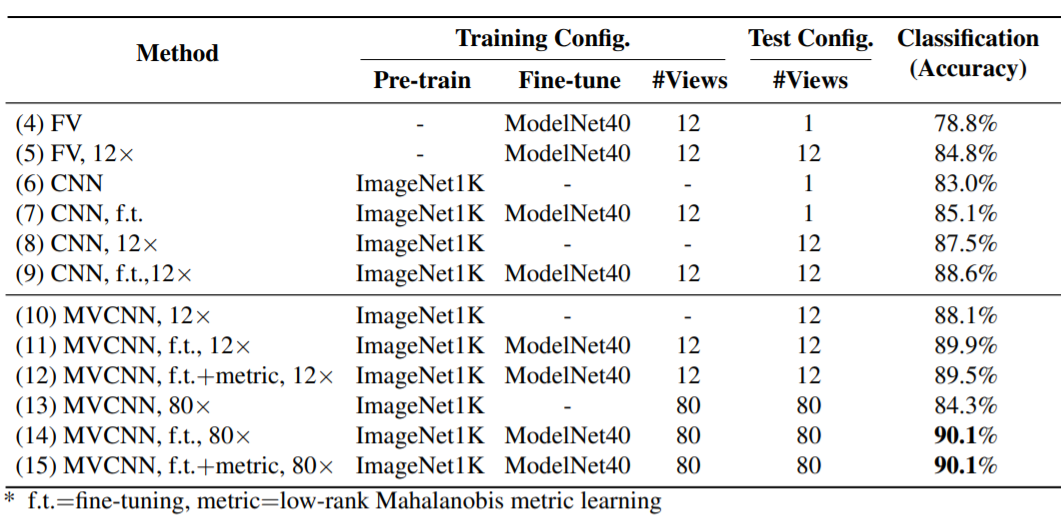
\includegraphics[width=0.8\textwidth]{images/MVCNN_results_table.png}
    \caption{ Classification and retrieval results. FV is another simpler approach described in the same paper that describes MVCNNs based on Fisher Vectors.}
    \label{fig:MVCNN_results_table}
\end{figure}

\begin{figure}[ht]
    \centering
    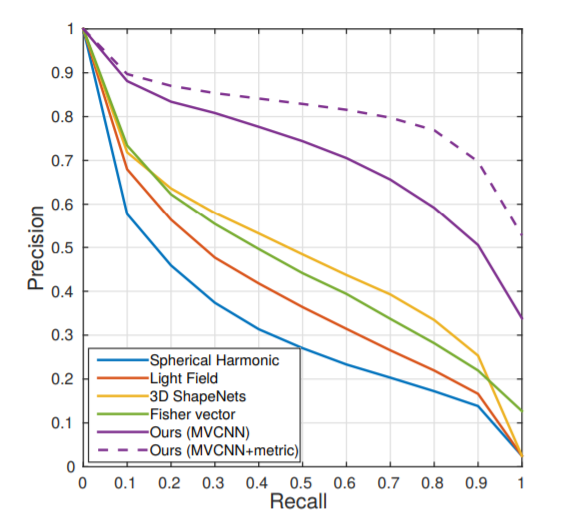
\includegraphics[width=0.5\textwidth]{images/MVCNN_prec_rec_curve.png}
    \caption{ Retrieval precision-recall curves.}
    \label{fig:MVCNN_prec_rec_curve}
\end{figure}

\paragraph{Saliency map among views}
Since this approach learns to aggregate views in a single network it is possible to trace back to the influence of the different views on the MVCNN output score $F_c$ for its ground truth class $c$. For each 3D shape $S$ and its relative views $\{I_1, I_2, ... I_K\}$ we can compute $w$ of the following equation using backpropagation

\begin{equation}
    [w_1, w_2, ... w_K] = \bigg[
    \frac{\partial F_c}{\partial I_1}\Bigr|_{\substack{S}},
    \frac{\partial F_c}{\partial I_2}\Bigr|_{\substack{S}},
    ... 
    \frac{\partial F_c}{\partial I_K}\Bigr|_{\substack{S}}
    \bigg]
\end{equation}

and obtain saliency maps for individual views. Some examples are reported in figure \ref{fig:MVCNN_saliency}.

\begin{figure}[ht]
    \centering
    \captionsetup{width=.9\linewidth}
    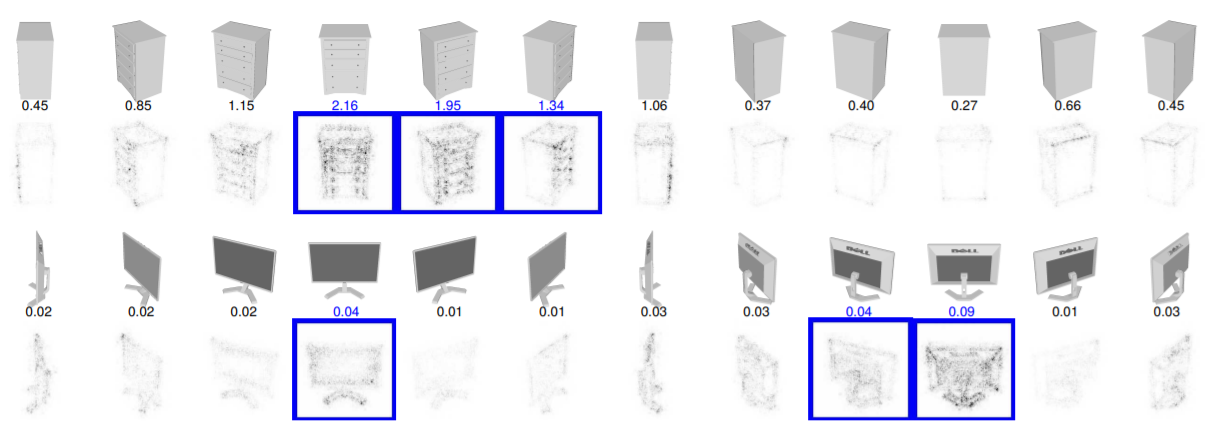
\includegraphics[width=0.9\textwidth]{images/MVCNN_saliency.png}
    \caption{Top three views with the highest saliency are highlighted in blue and the relative magnitudes of gradient energy for each view is
shown on top. The saliency maps are computed by back-propagating the gradients of the class score onto the image via the view-pooling
layer. Notice that the handles of the dresser and of the desk are the most discriminative features. (Figures are enhanced for visibility.)}
    \label{fig:MVCNN_saliency}
\end{figure}



% possibili approfondimenti:
%- Phong reflection model (https://users.cs.northwestern.edu/~ago820/cs395/Papers/Phong_1975.pdf)
%- Learning-based Multiple Pooling Fusion (https://s3.ap-northeast-2.amazonaws.com/journal-home/journal/jips/fullText/302/13.pdf)
% Saliency map (https://arxiv.org/pdf/1312.6034.pdf)
 



